\section{Contact and Rolling}

\subsection{Rigid bodies in contact}
\blue{Complete in "Rolling motion"}

\subsection{Rolling motion}
\blue{Complete in "Rolling motion"}

\subsection{Rolling on curved surfaces}
\blue{Complete in "Rolling motion"}

\subsection{\red{Applications}}
    \subsubsection{\red{Bearings}}
    \red{This topic is in L27, slides 13-14, include information in Fig \ref{fig:AppBearings}. Pictures are from this book \url{https://i-share-uiu.primo.exlibrisgroup.com/permalink/01CARLI_UIU/gpjosq/alma99955068260305899}}. Application for "Rolling on curved surfaces".

    \begin{figure}[h!]
        \centering
        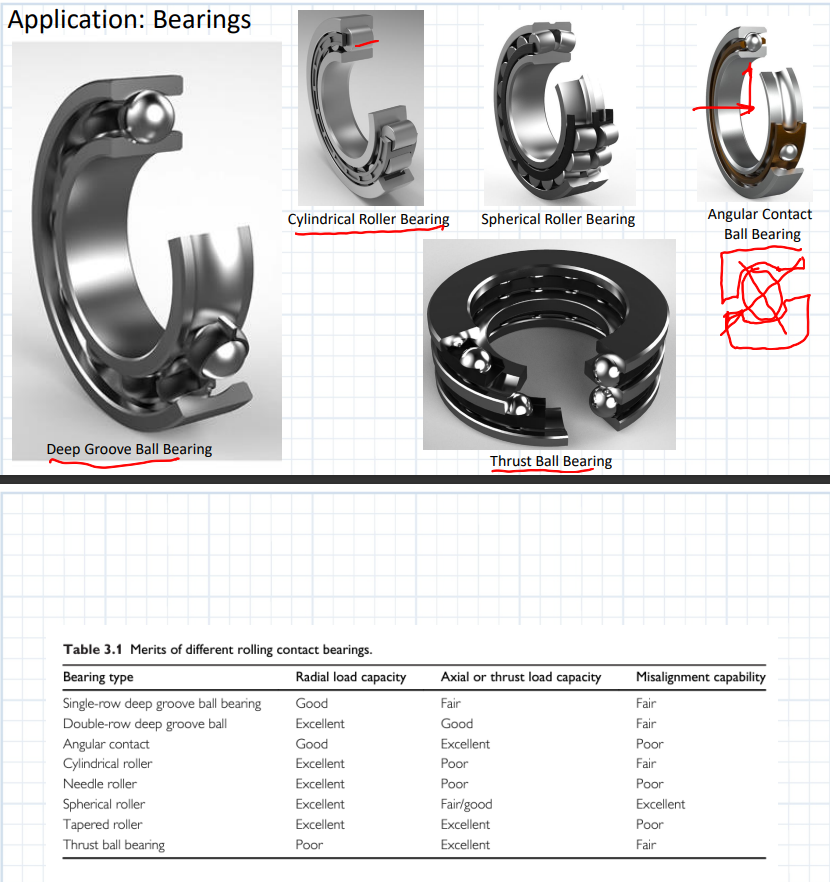
\includegraphics{ContactRollingFigs/AppBearings.png}
        \caption{From L27, slides 13-14}
        \label{fig:AppBearings}
    \end{figure}

